%!TEX root = ../Main.tex

\chapter{Genetic map of \textit{Yr15} with RNA-Seq}
\chaptermark{Genetic map of \textit{Yr15}}
\label{yr15}
%This section describes in detail than the paper of \citet{Ramirez-Gonzalez-2014}
 
%Breeding importance of \textit{Yr15} and original source (an introgression of \textit{T. diccocoides}). 
Wheat breeding programs aim to improve the wheat lines available for production.
One of the traits desired in an elite line is the resistance to pathogens, such as \textit{Puccinia striiformis} f. sp.  \textit{tritici}, the fungi responsible of yellow rust.
A source of resistance genes is are introgressions from other species, such as \textit{Triticum diccocides}. 
In the University of Sydney a collection of \glspl{nil} with introgressions to several Yellow Rust resistance genes on a susceptible background were developed \citep{Wellings1998}. 
On this chapter the NIL for the \textit{Yr15} locus is used to produce a mapping population to improve diagnostic markers. 

%TODO: Paragraph explaining NILs


Line selection can be done with molecular markers that can be used to test if certain allele is present in a line, without the need to do a phenotype.
To find which regions are linked to a trait the use of $F_{2}$ mapping populations is a common practice.
The population is produced by crossing two homozygous parents ($P_1$ and $P_{2}$) with different alleles, A/A (dominant) and a/a (recessive).
When the trait is dominant and has a mendelian segregation, the $F_1$ population show the dominant trait, as it has a copy of each allele (A/a). 
The $F_1$ is then self-crossed to and the population segregates with a ration 1:2:1, dominant:heterozygous:recessive respectively.
This generates a population with a phenotype ratio of 3:1 (dominant:recessive), since the effect of the recessive allele is masked by the dominant gene (\citealt{VanOoijen2013}; Figure \ref{fig:yr15:f2schematic}).  

\begin{SCfigure}
  \centering
    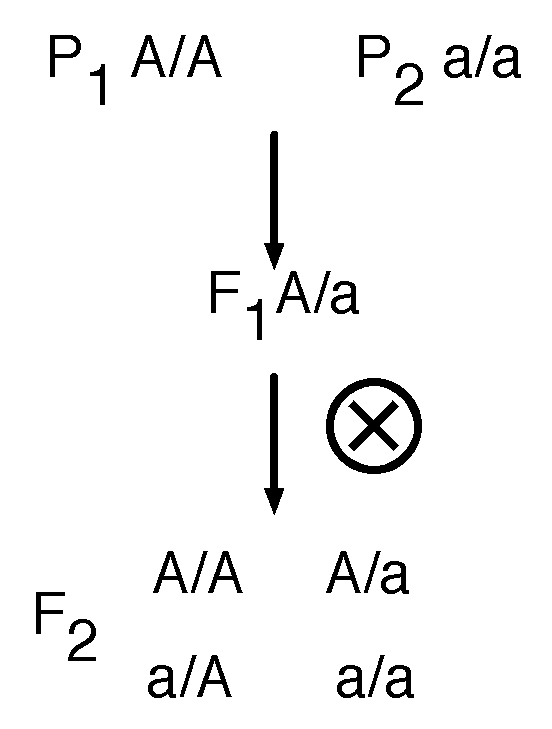
\includegraphics[width=0.4\textwidth]{Yr15/Figures/population/F2schematic.pdf}
  \caption{The cross of two homozygous parents, $P_{1}$ and $P_{2}$, with a dominant and a recessive allele of a gene produce an heterozygous $F_{1}$. The $F_{1}$ crossed with itself produce a segregating $F_{2}$ population with a 1:2:1 ratio (A/A:A/a:a/a). The upper and lower cases represent dominant and recessive alleles  }. 
  \label{fig:yr15:f2schematic}
\end{SCfigure}


\gls{bsa} consists on pooling the DNA of individuals with contrasting phenotypes \citep{Michelmore1991} on a segregating population. 
The bulks show as heterozygous except for the region that is linked to the trait of interest. 
This approach can be used to identify SNPs using High Throughput Sequencing, such as: exome capture \citep{Hodges2007}, RNA-Seq \citep{Pickrell2010}, whole genome resquencing \citep{Schneeberger2009}, among others. 


\begin{figure}
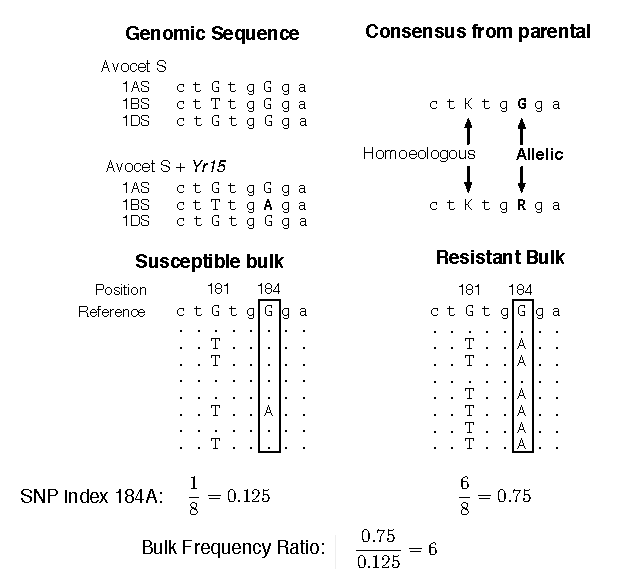
\includegraphics[width=1\textwidth]{Yr15/Figures/bfr.pdf}
\caption{Illustration of a non-informative homoeologous SNP (G181T) present in both parental lines, and an informative allelic SNP (G184A), only present in the resistant progenitor Avocet S + Yr15. The consensus sequences from the parental genotypes include this information in the form of ambiguity codes (K and R, respectively). In the bulks, the individual reads align across the reference sequence, with matches indicated by dots, and polymorphisms at positions 181 and 184 indicated by the corresponding nucleotide variants at those positions. The SNP index is calculated as the frequency of the informative allelic SNP in each bulk. The Bulk Frequency Ratio is the quotient of the resistant and susceptible bulk SNP Indexes. Figure previously published in \citet{Ramirez-Gonzalez2015c}. }
\label{fig:yr15:bfr}
\end{figure}


To Call for SNPs from RNA-Seq a reference transcriptome is used as target when aligning the reads. 
The \gls{bfr} methodology can work on organisms has more than one pseudo genome and that the genes are not necessarily fully characterised independently among homoeologues or paralogues, you can have in a single reference collapsing similar regions. 
The UniGenes database, from NCBI, contains the genes of each species, with all the variations of each gene automatically collapsed and represented as with the longest \acrshort{cdna} \citep{PontiusJUWagnerL2002}. 
The \acrshort{ucw}  genes described in \citet{Krasileva2013} contains 94,177 models from tetraploid and hexaploid wheat, assembled and phased to separate different homoeologues. 
Both gene sets are complement each other, however, the \acrshort{ucw} gene models should provide an improved alignment, since the different homoeologues aren't merged in a single model, a possible side effect of the UniGene pipeline. 

Homoeologous variants, as exemplified by the G$>$T variant at position 181; K in consensus (Figure \ref{fig:yr15:bfr}), will produce the same ambiguity code for both parental consensus sequences and can therefore be excluded. 
Real allelic SNPs between the parental genotypes, exemplified by the G$>$A variant at position 184; R in consensus, are distinguished by the presence in one, but not the other parental consensus sequence. 
The allelic SNPs are then examined further with the alignments of the bulks to identified the SNPs that are enriched on the resistant plants.
The SNP index is the proportion of times an alternative allele is observed over the coverage at certain, in the example the the susceptible bulk has an SNP index of $1/8=0.125$ and $6/8=0.75$ for the resistant bulk \citep{Takagi2013a}. traditional
The \acrshort{bfr} are then calculated by dividing the SNP Index of sample containing the target phenotype (resistance) over the sample without the trait (susceptible), on the example is $0.75/0.125=6$.  
A high BFR suggests that the \acrshort{snp} is linked to the target trait \citep{Trick2012}. 


Finally, the best candidate SNPs where selected to produce a genetic map which lead to a triplet of markers diagnostic to the target locus. 

The steps described in this chapter were first published in \citet{Ramirez-Gonzalez2015c} and the results of this chapter are published in \citet{Ramirez-Gonzalez2015b}.

\section{Mapping population}


\begin{figure}
%\begin{wrapfigure}[17]{R!}{7cm}
    \centering
     
     \begin{subfigure}[b]{0.4\textwidth}
        \caption{}
        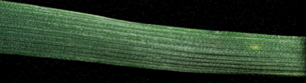
\includegraphics[width=1\textwidth]{Yr15/Figures/population/Yr15Photo.png}
        \label{fig:yr15.yr15Photo}
    \end{subfigure}
    ~
    \begin{subfigure}[b]{0.4\textwidth}
        \caption{}
        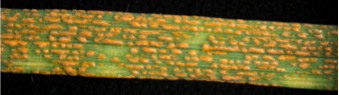
\includegraphics[width=1\textwidth]{Yr15/Figures/population/AVSPhoto.png}
        \label{fig:yr15:avsPhoto}
    \end{subfigure}

     \begin{subfigure}[b]{0.8\textwidth}
     \caption{}
        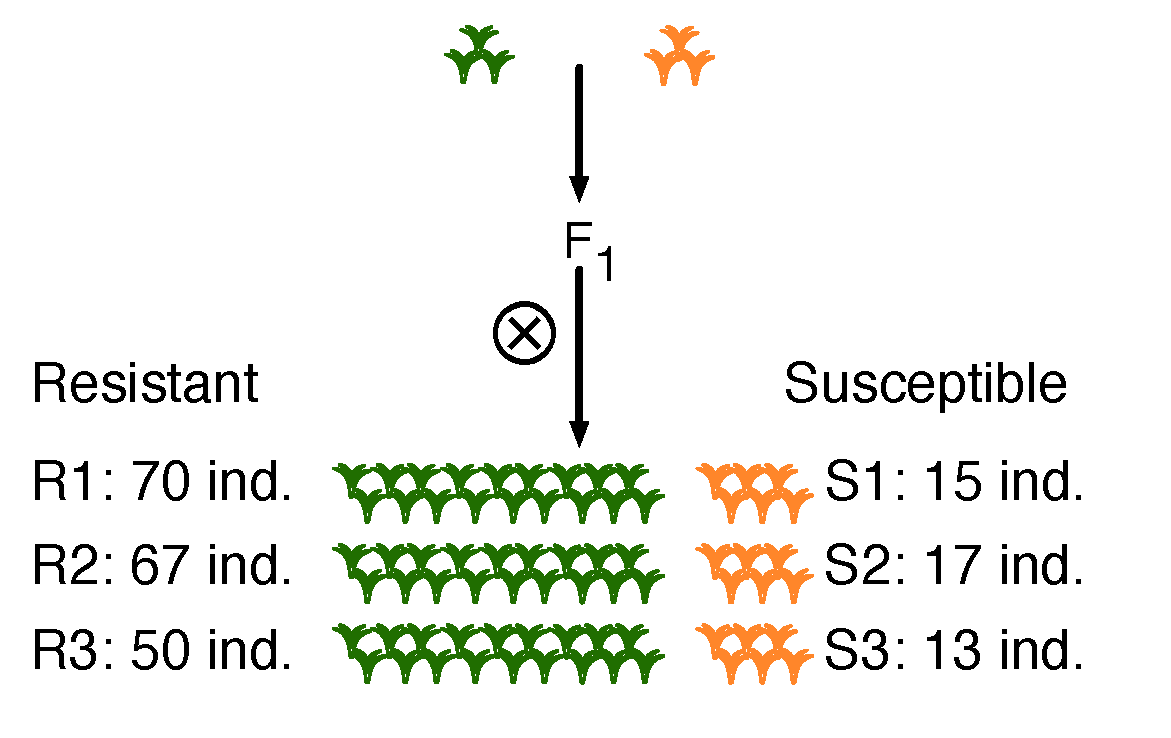
\includegraphics[width=1\textwidth]{Yr15/Figures/population/F2Population.pdf} 
    \label{fig:yr15:f2}
	\end{subfigure}

    \caption{Response of (\subref{fig:yr15.yr15Photo}) Avocet + \textit{Yr15} and (\subref{fig:yr15:avsPhoto}) Avocet when inoculated with \textit{Puccinia striiformis} f. sp.  \textit{tritici} at the three leaf stage. (\subref{fig:yr15:f2}) The phenotype of the $F_{2}$ population was used to produce 6 bulks, 3 resistant and 2 susceptible. The RNA was pooled in bulks accordingly. Adapted from \citep{Ramirez-Gonzalez2015b}}

%\end{wrapfigure}
\end{figure}

The population was developed by crossing the resistant line \gls{yr15} \citep{Wellings1998}, Figure \ref{fig:yr15.yr15Photo}, to the susceptible line \gls{avs}, Figure \ref{fig:yr15:avsPhoto}. 
\acrshort{yr15} is a \gls{nil} of a 6th generation \gls{bc} and the \acrshort{avs} background is highly succeptible to yellow rust, hence the resistance is coffered by the \acrshort{yr15} locus. 
$F_{2}$ seeds from tree independent $F_{1}$ plants where sown and tissue was collected, before the fungal inoculation to avoid the effect of the response on the gene expression.  
The plants were challenged at the three leaf stage as it is know that \textit{Yr15} confers resistance in seedlings \citep{Gerechter-Amitai1989}.
The expected segregation on an $F_{2}$ population is 3:1 (resistant:susceptible), since \textit{Yr15} is a dominant gene.
From the 232 plants in the $F_{2}$ population that germinated, 187 were resistant and 45 were susceptible, which deviates slightly from the expected ratio ($\chi^{2}=0.049$).
Segregation distortion has been shown for the same \textit{Yr15} donnor \citep{Randhawa2009}, however the decresed number of succeptible plants can be explained by escapes in the virulence essays (i.e. plants scored as resistant without the \textit{Yr15} locus).   For this study we extracted DNA from individual plants in the $F_{2}$ population and we bulked RNA on 6 different bulks: 3 resistant and, 3 succeptible ( Figure \ref{fig:yr15:f2}). 

\section{Sequencing and mapping} 

\begin{table}
\centering
\caption{Arrangement and number of sequenced base pairs per sample. }
\label{tab:yr15:reads}
\begin{tabular}{rrccccc}
\toprule
Library & name & Bar code & Lane   &  Reads (\e{8} bp)\\ 
\midrule
LIB1715 & Bulk R1 & ATCACG & 1 	& 0.77\\
LIB1716 & Bulk R2 & TAGCTT & 1 		& 1.20\\
LIB1717 & Bulk R3 & ACTTGA & 2 	& 0.96  \\ 
LIB1718 & Bulk S1 & GGCTAC & 2 	& 1.64   \\ 
LIB1719 & Bulk S2 & CGTACG & 2 	& 1.49  \\ 
LIB1720 & Bulk S3 & GTGGCC & 1 	&1.88  \\ 
LIB1721 & AvocetS & N/A & 3 		& 4.13 \\ 
LIB1722 & AvocetS + \textit{Yr15} & N/A & 4 	& 3.99  \\ 
\bottomrule
\end{tabular}
\end{table}


RNA-Seq was used to avoid sequencing the non-coding regions and reduce the search space.  
The sequencing of the bulks and the parents were done on a single Illumina Hi-Seq2000 each.
The bulks were multiplexed and sequenced on a third of a lane each, as shown on Table \ref{tab:yr15:reads}. 
To ensure that the quality of the sequencencing was good, \verb|fastqc-0.10| \citep{fastqc}  was run with its default parameters in each one of the fastq files.  
The GC content was around 52\% in all the samples (Appendx \ref{App:AppendixQCGC}), which is expected as the sample should be of coding regions, and for wheat the reported GC content in genes is around 55\%.  
The quality of the reads is fairly consistent, in general dropping after the base 80 across the samples (Appendix \ref{App:AppendixQCRead}). 


%!TEX root = ../../Main.tex
\begin{sidewaystable}
\centering
\caption{Number of genes with a coverage over 20x, 10x and at least one read (\ensuremath{>}0x). }
\label{app:seqAlnCov}
\begin{localsize}{10}{11}

\begin{tabular}{llrrrrrr|rrrr|rr}
\toprule
          &             & \multicolumn{6}{c}{Bulks} & \multicolumn{4}{c}{Bulk  mixes} & \multicolumn{2}{c}{Progenitors}        \\
 Coverage & Reference   & R1     & R2     & R3     & S1     & S2     & S3     & R1+R2       & S1+S2  & R1+R2+R3 & S1+S2+S3 & \textit{Yr15}        & AVS     \\
 \midrule
 20x      & UCW         & 16,434 & 27,871 & 27,223 & 32,287 & 28,669 & 34,898 & 33,968      & 41,019 & 40,985   & 47,507   & 36,808      & 42,248  \\
          &             & 17\%    & 30\%    & 29\%    & 34\%    & 30\%    & 37\%    & 36\%         & 44\%    & 44\%      & 50\%      & 39\%         & 45\%     \\
          & UniGene v60 & 9,643  & 16,182 & 15,222 & 19,549 & 17,397 & 20,567 & 20,219      & 25,270 & 24,598   & 29,052   & 22,107      & 25,842  \\
          &             & 17\%    & 28\%    & 27\%    & 34\%    & 31\%    & 36\%    & 36\%         & 44\%    & 43\%      & 51\%      & 39\%         & 45\%     \\
 \midrule
 10x      & UCW         & 27,371 & 38,282 & 37,777 & 42,658 & 38,999 & 44,610 & 43,266      & 49,473 & 49,182   & 54,781   & 46,356      & 50,760  \\
          &             & 29\%    & 41\%    & 40\%    & 45\%    & 41\%    & 47\%    & 46\%         & 53\%    & 52\%      & 58\%      & 49\%         & 54\%     \\
          & UniGene v60 & 16,201 & 22,948 & 22,130 & 26,200 & 24,130 & 26,914 & 26,318      & 30,579 & 29,857   & 33,557   & 28,044      & 31,095  \\
          &             & 28\%    & 40\%    & 39\%    & 46\%    & 42\%    & 47\%    & 46\%         & 54\%    & 52\%      & 59\%      & 49\%         & 55\%     \\
 \midrule
 \ensuremath{>}0x      & UCW         & 68,302 & 72,484 & 72,957 & 74,694 & 73,290 & 75,201 & 74,397      & 77,093 & 76,715   & 78,796   & 76,275      & 77,080  \\
          &             & 73\%    & 77\%    & 77\%    & 79\%    & 78\%    & 80\%    & 79\%         & 82\%    & 81\%      & 84\%      & 81\%         & 82\%     \\
          & UniGene v60 & 40,717 & 42,489 & 42,595 & 43,625 & 43,059 & 43,748 & 43,393      & 44,655 & 44,364   & 45,392   & 43,732      & 44,596" \\
          &             & 71\%    & 75\%    & 75\%    & 77\%    & 76\%    & 77\%    & 76\%         & 78\%    & 78\%      & 80\%      & 77\%         & 78\%     \\
\bottomrule
\end{tabular}

\end{localsize}
\end{sidewaystable}



\begin{figure}
\centering
\begin{subfigure}{0.29\textwidth}
    \caption{}
     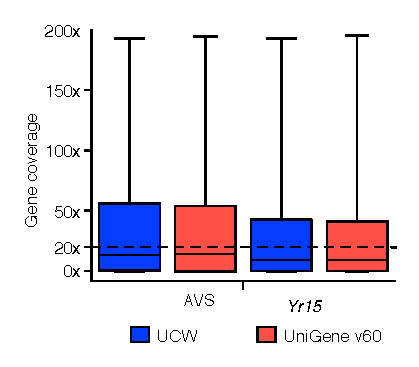
\includegraphics[width=1\textwidth]{Yr15/Figures/CoveragePerGene.pdf} 
    \label{fig:yr15:covPerGene}
\end{subfigure}
~
\begin{subfigure}{0.5\textwidth}
    \caption{}
    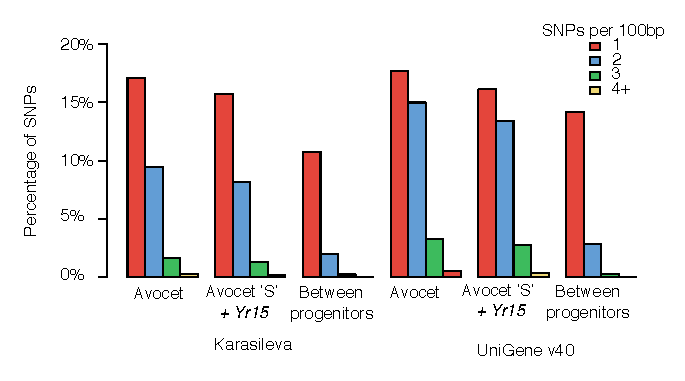
\includegraphics[width=1\textwidth]{Yr15/Figures/PercentageOfSnps.pdf} 
    
    \label{fig:yr15:SNPper}
\end{subfigure}

\caption{(\subref{fig:yr15:covPerGene}) Box plot distribution of the gene coverage of the parent reads (\acrshort{avs} and \acrshort{yr15}) across the UCW (blue) and the UniGene (red) gene models. The dashed line represents the 209 minimum coverage required for SNP calling. The full line represents the average coverage across all gene models. (\subref{fig:yr15:SNPper}) Percentage of genes exhibiting SNPs across references. The number of \acrshort{snp}s between the parent reads and the corresponding references was calculated (per 100 bp, rounded). The ‘between-parents’ category corresponds to putative SNPs when comparing the consensus sequence between \acrshort{avs} and \acrshort{yr15} Adapted from \citet{Ramirez-Gonzalez2015b} }
\end{figure}


When the analysis was started, the draft genome and the corresponding annotation where not not release yet, hence gene models where used. 
All the samples where aligned to the Unigenes v60 (56,954 genes) and the gene models from UCW \citep{Krasileva2013} using \verb|BWA 0.5.9| \citep{Li2009}. 
The alignment provided showed that a few genes were overly expressed, however we still have have 22,107 and 36,808 genes, on the Unigenes and the UCW gene set respectivley,  with a coverage greater than 20x in the progenitor with \textit{Yr15}. 
Both gene sets performed similarly in terms of the percentage of genes with reads and percentage of aligned reads. 
For \gls{avs} and \gls{yr15}, the percentage of genes with a coverage of at least $20x$ is $45\%$ and $39\%$ respetively across both references (Figure \ref{fig:yr15:covPerGene}).
Since each individual bulk has a lower coverage, the susceptible and resistant reads were merged \textit{in silico} as: (i) susceptible bulks 1 with 2 (S1 + S2) and resistant bulks 1 with 2 (R1 + R2) and (ii) all the susceptible (S1 + S2 + S3) and resistant bulks (R1 + R2 + R3). 
The merged samples increased the percentage of genes with coverage over 20x  to 44\% and 50\% in the resistant and susceptible bulks (Table \ref{app:seqAlnCov}), which is close to the coverage from the progenitors.

\section{SNP Calling}

The \acrshort{snp} calling was done on positions with a coverage of at least $20x$ on the progenitor lines against the gene reference. The \acrshort{avs} progenitor had roughly $3\%$ more genes with polymorphisms than \acrshort{yr15}, consistent with the difference in coverage, suggesting that with a higher coverage we could recover more \acrshort{snp}s from \acrshort{yr15}.
The UniGenes have a higher number of \acrshort{snp}s because the \acrshort{ucw} gene models have a higher number of monomorphic genes when compared to the UniGenes. (Figure {\ref{fig:yr15:SNPper}}; Table \ref{app:yr15:cntSNP100bp}). 
The difference in the number of relative monomorphic SNPs between references can be explained by the fact that the UniGenes have homoeologues can be represented as a single sequence, as opposed to the UCW set which are homoeologue-specific, improving the mapping to the correct homoeologue in the genes from the UCW set over the UniGenes.

%!TEX root = ../../Main.tex
\begin{table}
\caption{ Count of SNPs per 100 bp on genes with at least 20x coverage. }
\centering
\label{app:yr15:cntSNP100bp}
\begin{localsize}{10}{12}
\begin{tabular}{lrrrrrrr}
\toprule
 SNPs  & \multicolumn{3}{c}{UCW}  &  &  \multicolumn{3}{c}{UniGene v60 }                                 \\
 \cline{2-4}
 \cline{6-8}
\pbox{1cm}{per 100bp}         & AVS   & \pbox{1.5cm}{\centering AVS+ \textit{Yr15}} & \pbox{1.8cm}{\centering Between progenitors} &      & AVS         & \pbox{1.5cm}{\centering AVS+ \textit{Yr15}} & \pbox{1.8cm}{\centering Between progenitors} \\
\midrule
 0               & 67, 389       & 70,338 & 81,921             &      & 36,210       & 38,339      & 47,097               \\
                 & 71.6\% & 74.7\%      & 87.0\%               &      & 63.6\%       & 67.3\%      & 82.7\%               \\
 \midrule
 1               & 16,111 & 14,770      & 10,107               &      & 10,058       & 9,175       & 8,061                \\
                 & 17.1\% & 15.7\%      & 10.7\%               &      & 17.7\%       & 16.1\%      & 14.2\%               \\
 \midrule
 2               & 8,904  & 7,676       & 1,893                &      & 8,529	         & 7,648       & 1,621                \\
                 & 9.5\%  & 8.2\%       & 2.0\%                &      & 15.0\%       & 13.4\%      & 2.9\%                \\
 \midrule
 3               & 1,517  & 1,192       & 215                  &      & 1,870        & 1,568       & 59       \\
                 & 1.6\%  & 1.3\%       & 0.2\%                &      & 3.3\%        & 2.8\%       & 0.3\%                \\
 \midrule
 4+              & 253    & 198         & 38                   &      & 287          & 224         & 16                  \\
                 & 0.3\%  & 0.2\%       & 0.0\%                &      & 0.5\%        & 0.4\%       & 0.0\%                \\
\bottomrule
\end{tabular}
\end{localsize}
\end{table}

Both gene sets were done from varieties different to \acrshort{avs} and are likely to be incomplete, hence we set a low threshold of at least 20\% of the observed nucleotides on any position to call an \acrshort{snp}. 
To represent cases were more than one consensus base is called we use \gls{iuapc} codes (\citet{Cornish-Bowden1985}; Section \ref{lit:ambiguity}; Figure \ref{fig:yr15:bfr}).  
To focus the analysis on informative \acrshort{snp}s, the common varietal SNPs and variations between homoeologues were removed by finding the cases when the consensus call on both progenitors is the same. 
The \acrshort{snp}s that are unique to a single parental were examined in detail. 
There are 66,426 putative SNPs across 16,022 (17\%) \acrshort{ucw} genes and 52,262 \acrshort{snp}s on 11,056 UniGenes (19.4\%; Figure \ref{fig:yr15:geneCount}).  

\begin{SCfigure}
    %\centering
    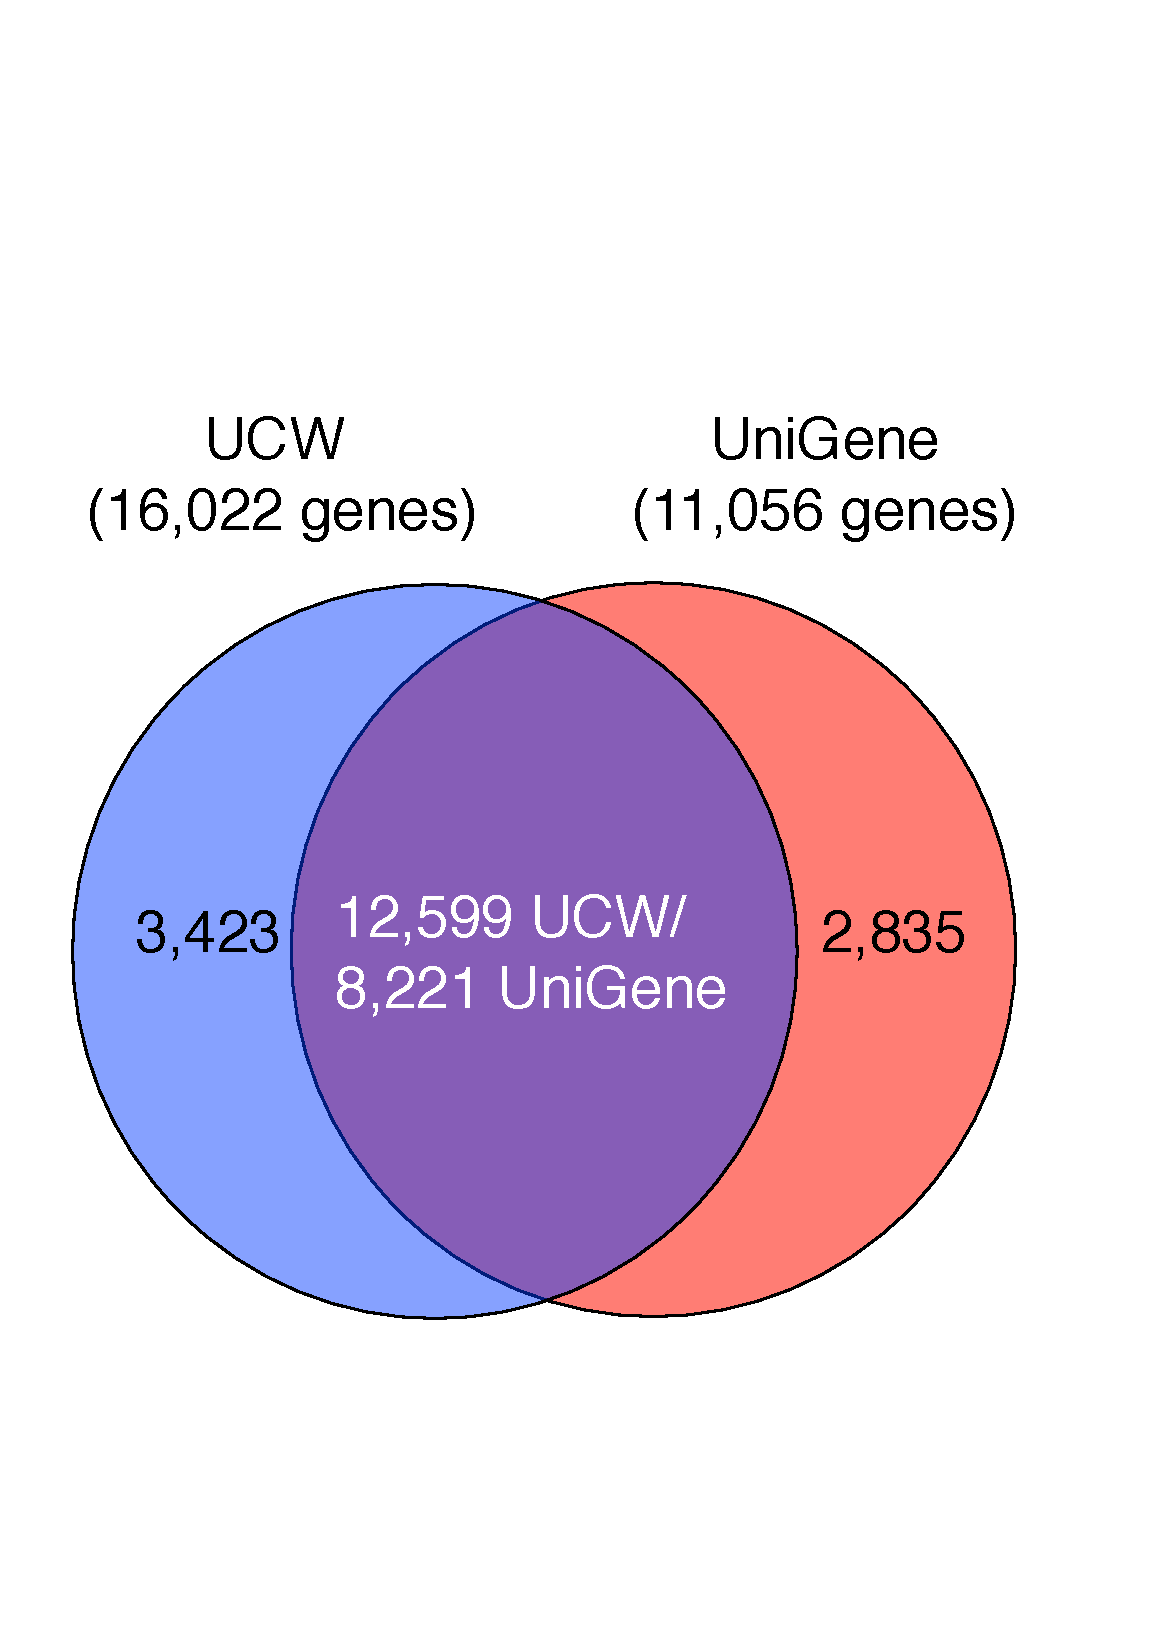
\includegraphics[width=0.4\textwidth]{Yr15/Figures/geneCounts.pdf} 
    \caption{Gene models with putative SNPs in common between the UCW and UniGenes reference. The intersection represnts the genes that are common in both sets. Adapted from \citet{Ramirez-Gonzalez2015b}}
    \label{fig:yr15:geneCount}
\end{SCfigure}

%!TEX root = ../../Main.tex
\begin{table}
\centering
\caption{ Number of genes assigned to the wheat chromosome arm CSS scaffolds \citep{Mayer2014} using the best hit from BLAT \citep{Kent2002} }
\label{tab:yr15:genesToCSS}
\begin{localsize}{10}{12}
\begin{tabular}{lrrr}
\toprule
 \pbox{2.2cm}{Wheat \\Chromosome Arm}    & UCW (94,177)    & UniGene v60 (56,954)   & Total (151,131)   \\
\midrule
 1AL                     & 3,251 (3.45\%)   & 1,404 (2.47\%)          & 4,655 (3.08\%)     \\
 1AS                     & 1,366 (1.45\%)   & 560 (0.98\%)            & 1,926 (1.27\%)     \\
 1BL                     & 2,610 (2.77\%)   & 1,280 (2.25\%)          & 3,890 (2.57\%)     \\
 1BS                     & 1,487 (1.58\%)   & 693 (1.22\%)            & 2,180 (1.44\%)     \\
 1DL                     & 997 (1.06\%)     & 1,057 (1.86\%)          & 2,054 (1.36\%)     \\
 1DS                     & 753 (0.80\%)     & 687 (1.21\%)            & 1,440 (0.95\%)     \\
 \midrule
 2AL                     & 3,491 (3.71\%)   & 1,460 (2.56\%)          & 4,951 (3.28\%)     \\
 2AS                     & 2,305 (2.45\%)   & 974 (1.71\%)            & 3,279 (2.17\%)     \\
 2BL                     & 3,658 (3.88\%)   & 1,546 (2.71\%)          & 5,204 (3.44\%)     \\
 2BS                     & 2,790 (2.96\%)   & 1,139 (2.00\%)          & 3,929 (2.60\%)     \\
 2DL                     & 1,098 (1.17\%)   & 1,069 (1.88\%)          & 2,167 (1.43\%)     \\
 2DS                     & 796 (0.85\%)     & 833 (1.46\%)            & 1,629 (1.08\%)     \\
 \midrule
 3AL                     & 2,135 (2.27\%)   & 978 (1.72\%)            & 3,113 (2.06\%)     \\
 3AS                     & 1,543 (1.64\%)   & 718 (1.26\%)            & 2,261 (1.50\%)     \\
 3B                      & 6,559 (6.96\%)   & 2,839 (4.98\%)          & 9,398 (6.22\%)     \\
 3DL                     & 915 (0.97\%)     & 938 (1.65\%)            & 1,853 (1.23\%)     \\
 3DS                     & 412 (0.44\%)     & 450 (0.79\%)            & 862 (0.57\%)       \\
 \midrule
 4AL                     & 3,393 (3.60\%)   & 1,335 (2.34\%)          & 4,728 (3.13\%)     \\
 4AS                     & 2,011 (2.14\%)   & 817 (1.43\%)            & 2,828 (1.87\%)     \\
 4BL                     & 2,119 (2.25\%)   & 898 (1.58\%)            & 3,017 (2.00\%)     \\
 4BS                     & 1,946 (2.07\%)   & 892 (1.57\%)            & 2,838 (1.88\%)     \\
 4DL                     & 1,069 (1.14\%)   & 945 (1.66\%)            & 2,014 (1.33\%)     \\
 4DS                     & 800 (0.85\%)     & 699 (1.23\%)            & 1,499 (0.99\%)     \\
 \midrule
 5AL                     & 2,640 (2.80\%)   & 1,132 (1.99\%)          & 3,772 (2.50\%)     \\
 5AS                     & 963 (1.02\%)     & 407 (0.71\%)            & 1,370 (0.91\%)     \\
 5BL                     & 5,324 (5.65\%)   & 1,943 (3.41\%)          & 7,267 (4.81\%)     \\
 5BS                     & 1,360 (1.44\%)   & 591 (1.04\%)            & 1,951 (1.29\%)     \\
 5DL                     & 2,067 (2.19\%)   & 1,688 (2.96\%)          & 3,755 (2.48\%)     \\
 5DS                     & 620 (0.66\%)     & 614 (1.08\%)            & 1,234 (0.82\%)     \\
 \midrule
 6AL                     & 2,397 (2.55\%)   & 896 (1.57\%)            & 3,293 (2.18\%)     \\
 6AS                     & 2,285 (2.43\%)   & 936 (1.64\%)            & 3,221 (2.13\%)     \\
 6BL                     & 1,564 (1.66\%)   & 820 (1.44\%)            & 2,384 (1.58\%)     \\
 6BS                     & 1,308 (1.39\%)   & 731 (1.28\%)            & 2,039 (1.35\%)     \\
 6DL                     & 1,399 (1.49\%)   & 1,050 (1.84\%)          & 2,449 (1.62\%)     \\
 6DS                     & 870 (0.92\%)     & 680 (1.19\%)            & 1,550 (1.03\%)     \\
 \midrule
 7AL                     & 1,918 (2.04\%)   & 849 (1.49\%)            & 2,767 (1.83\%)     \\
 7AS                     & 1,717 (1.82\%)   & 764 (1.34\%)            & 2,481 (1.64\%)     \\
 7BL                     & 1,592 (1.69\%)   & 776 (1.36\%)            & 2,368 (1.57\%)     \\
 7BS                     & 1,239 (1.32\%)   & 713 (1.25\%)            & 1,952 (1.29\%)     \\
 7DL                     & 2,040 (2.17\%)   & 1,301 (2.28\%)          & 3,341 (2.21\%)     \\
 7DS                     & 1,224 (1.30\%)   & 1,016 (1.78\%)          & 2,240 (1.48\%)     \\
 \midrule
 Assigned                & 80,031 (84.98\%) & 41,118 (72.20\%)        & 121,149 (80.16\%)  \\
\bottomrule
\end{tabular}
\end{localsize}
\end{table}

The high number of genes with \acrshort{snp}s was unexpected as a \acrshort{bc}6 \acrshort{nil} used for an $F_2$ mapping population expects to have $<1\%$ of the genetic background segregating. 
The both sets of gene models were aligned with BLAT \citep{Kent2002} to the Chinese Spring Chromosome arm survey sequence (CSS; \citealt{Mayer2014}); the alignment resulted on 80,031 (85.0\%) UCW gene models and 41,118 (72.2\%) UniGenes assigned to a chromosome arm (Table \ref{tab:yr15:genesToCSS}). 
The SNPs found in the mapped genes are evenly distributed across all the chromosomes (Figure \ref{fig:yr15:bfr0}), suggesting that the \acrlong{avs} (JIC, UK) used as parent in the $F_{2}$ is different to the \acrlong{avs} used for the \acrshort{yr15} \acrshort{nil} development (University of Sydney, Australia).  


To confirm that the \acrlong{avs} seed stocks from JIC are distinct to the stocks in Sydney  DNA from both stocks was procured and compared with the iSelect 90k wheat SNP chip. 
Between two independent \acrlong{avs} seeds from JIC only 58 out of 71,972 (0.08\%) valid assays were polymorphic. 
Nonetheless, ther are over 5,000 ($>7.5\%$) assays with polymorphisms between  JIC-\acrlong{avs} and \acrlong{avs} from Sydney. 
The different was not expected originally, but considering that the \acrlong{avs} seeds are coming from different stocks and the fact that in both countries commercial varieties with the same name had been released, it is not surprising. 


\section{Bulk Frequency Ratios}

The Bulk Frequency Ratio (BFR) algorithm (\citealt{Trick2012}; Figure \ref{fig:yr15:bfr}) on tetraploid wheat, was used to identify loci linked to the resistance provided by \textit{Yr15} in the segregating population.
Briefly, the consensus sequence for each of the progenitors is obtained from the pileups, allowing to call variants having 20\% of the bases as an alternative allele. 

\begin{figure}
	\centering
	\begin{subfigure}{0.4\textwidth}
	\caption{}
	\label{fig:yr15:bfr0}
	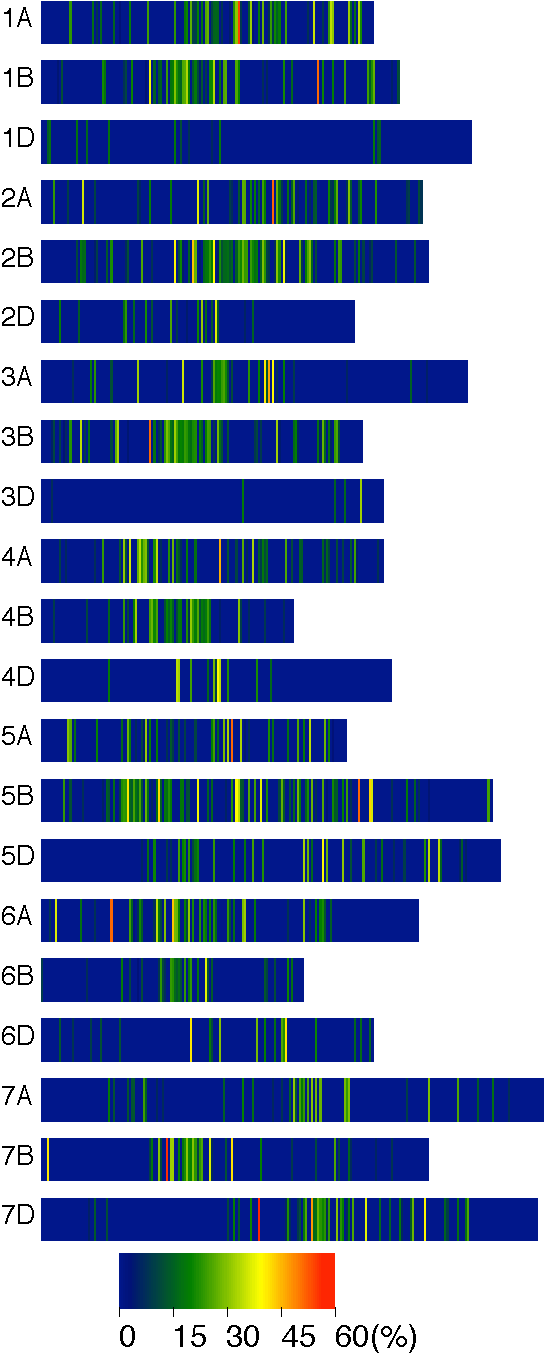
\includegraphics[height=0.55\textheight]{/Users/ramirezr/Documents/public_code/PhdThesis/Yr15/Figures/mapping/snpsBFR0.pdf}
	\end{subfigure}
	~
	\begin{subfigure}{0.45\textwidth}
	\caption{}
	\label{fig:yr15:bfr6}
	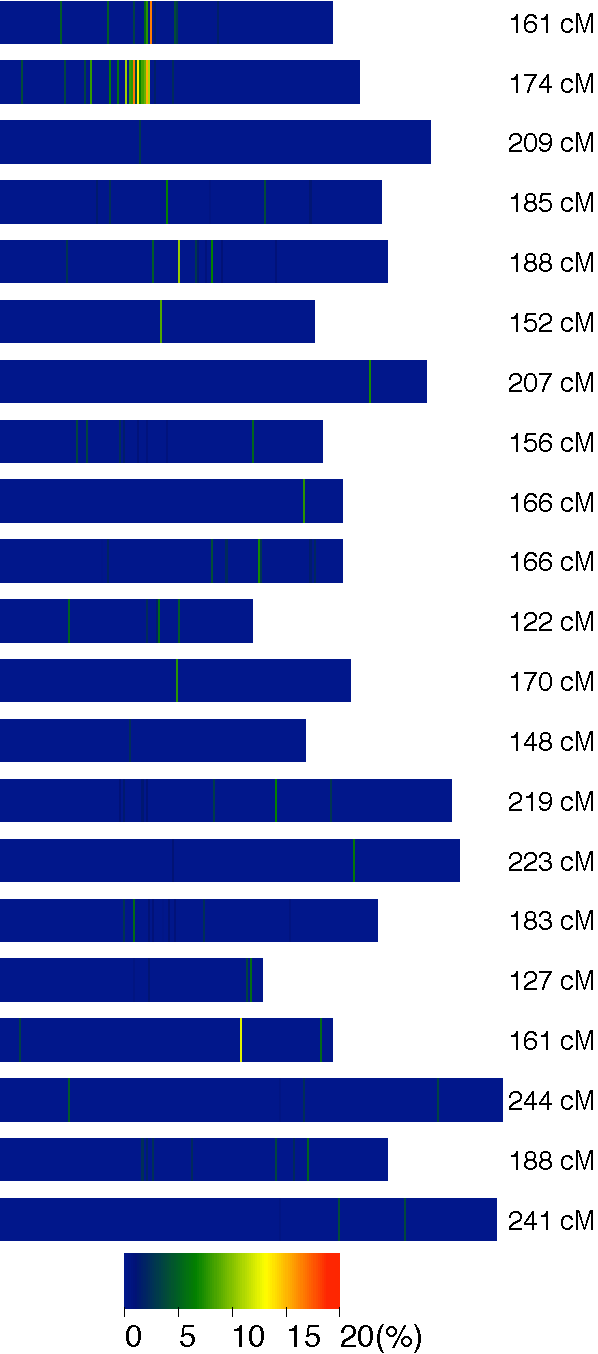
\includegraphics[height=0.55\textheight]{/Users/ramirezr/Documents/public_code/PhdThesis/Yr15/Figures/mapping/snpsBFR6.pdf}
	\end{subfigure}
	\caption{Genetic location of genes with SNPs between AVS and Yr15. The colour scale indicates the percentage of genes with SNPs per centi-Morgan (cM) across the 21 wheat chromosomes. The location of the genes was determined by the best alignment to the CSS scaffolds, and the location of these was determined by their position on a genetic map \citep{Wang2014} (\subref{fig:yr15:bfr0}). All the SNPS between progenitors. Note the lack of enrichment across any individual chromosome. (\subref{fig:yr15:bfr6}) SNPs with BFR$>$6. Note the enrichment in Chromosome 1B }
	\label{fig:yr15:bfrs:0-6}
\end{figure}

\section{\textit{In silico} mapping}
Mapping of the gene models to the IWGSC CSS \citet{Mayer2014} reference and the location of the SNPs using the genetic map from \citet{Wang2014}.

\section{Assay selection}. 
The selection criteria to decide which SNPs where selected to produce the genetic map: BFR$>$6, in the short arm of chromosome group 1 and from the \textit{Yr15} progenitor.

\section{Genetic map} 
\label{yr15:geneticMap}
The three versions of the genetic map: With a subset of the F\textsubscript{2} population

\section{Bioinformatic methods}

\subsection{Alignment reads to gene models}

The raw output from the Illumina HiSeq 2000 was processed with Casava v1.8 \citep{casavaBCL}. 
Lanes 1 and 2, containing multiplexed bulks (Table \ref{tab:yr15:reads}) was demultiplexed with a tolerance of 1 mismatch in the barcode. 
Lanes 3 and 4 contained the parental sequences without a barcode. 
The FastQ files where left compressed and in chunks of 40,000, as teh default for the BCL conversion pipeline from Casava to allow parallel processing in a cluster environment. 
The quality of the sequencing lanes was assessed with FastQC v0.10.1 \citep{fastqc}. 
The RNA-Seq reads were aligned with BWA 0.5.9 \citep{Li2009} to the wheat UniGene database v60 \citep{PontiusJUWagnerL2002} and to the UCW gene models \citep{Krasileva2013}, including the \textit{T. turgidum} and complementary ORFs \citep{MASWheat2013}.
The alignments where sorted and stored as single BAM files to have random access \citep{Li2009a}. 

%TODO: Snippet with submission of the alignments. 

\subsection{Bulk Frequency Ratios}

%To identify variant candidates, the methodology described in Trick et al. (2012) was used and extended to work with BAM files and to consider cases when a variant is completely absent from the parental sequences. The consensus from the two parents is called, allowing for ambiguities to take into account possible homoeo- logues when at least 20% of the bases differ from the reference. The consensus is stored with standard IUPAC codes (Cornish- Bowden, 1985). On the bases where the consensus is different between the parents, the bulk frequency ratio (BFR) was calculated as in Trick et al. (2012). The algorithm was imple- mented using Ruby on the top of BioRuby (Goto et al., 2010) and extending the functionality of bio-samtools (Ramirez-Gonzalez et al., 2012). The BFRs were calculated independently on each of the three comparisons (Bulk 1: S1–R1, Bulk 2: S2–R2 and Bulk 3: S3–R3) and with in silico mixes of bulks 1 and 2; and bulks 1, 2 and 3 produced by merging the BAM files using samtools (Li et al., 2009). A list was produced with all the scores in a table format containing the BFR, coverage, ratio of the SNP base and the the parent containing the SNP (Data S2–S4).

%The UniGenes, UCW gene models and the contigs containing the 46 977 genetically mapped SNPs from Wang et al. (2014) were aligned with BLAT (Kent, 2002) to the CSS scaffolds (IWGSC, 2014). To assign the genes to a specific scaffold, we selected the best hit from the BLAT alignment, provided that at least 60% of the gene was covered in the scaffold with at least 90% of identity. This selection criterion reduces the number of spurious hits in repetitive motifs in the gene and allows the assignment to a homoeologous chromosome even when the correct homoeologue is missing from the CSS scaffolds. The origin of the scaffold was used to assign a putative chromosome arm. In addition, the gene models were also aligned to the cDNA of Hordeum vulgare (International Barley Genome Sequencing Consortium, 2012) from Ensembl! Plants, release 16 (Kersey et al., 2012). The genetic position of the wheat contigs with SNPs was used to calculate the density of SNPs with a BFR > 6 and for all SNPs between AVS and Yr15. After selection using the criteria outlined in the results section, the selected genes were sorted by BFR in the mix between samples to select the top 50 SNPs for further validation via KASP markers.

%\section{Assembly of the transcriptome} 
%A comparison between thef known unigenes and the transcript from the progenitors. Since \textit{Yr15} comes from an introgression with \textit{T. diccocoides}, some novel transcripts can be extracted. Analysis of the gels from Mitaly? 

\section{Discussion} 
Remarks on how this techinque can be used to do fine-mapping and that if I were to start the project now I would  use exome capture or Ren-Seq. 

The references have changed since we started

There are new annotations, now we don't necessarily need to use unigenes anymore. 

Importance of genotyping everything used in an experiment

Mention other people using a similar strategy since this was published. 

We can use different techniques now (exome capture, ren-seq)

The markers are now used by our collaborators. 